\documentclass[10pt]{article}
\usepackage[letterpaper,margin=0.8in]{geometry}
\usepackage{amsmath,amssymb,booktabs,graphicx}
\usepackage[T1]{fontenc}
\usepackage{lmodern}
\usepackage[hidelinks]{hyperref}
\usepackage{xurl}
\setlength{\parindent}{0pt}\setlength{\parskip}{4pt}
\newcommand{\TailNumerator}{5869345}
\newcommand{\TailDenominator}{20037600}
\newcommand{\TailDecimal}{0.292916567}
\newcommand{\PairFraction}{0.573529412}
\newcommand{\HigherCount}{55}
\newcommand{\TieCount}{7}
\newcommand{\LowerCount}{40}

\makeatletter
\renewcommand{\maketitle}{\begin{center}{\Large\bfseries\@title\par}\vspace{5pt}\@author\qquad\@date\end{center}}
\makeatother
\title{Exact Label-Allocation Audit of Frobenius Splitting Scores}
\author{Anonymous}\date{30 October 2026}
\begin{document}\maketitle
\begin{abstract}
Using previously verified scores, we exactly count all 20037600 fixed-field
label assignments for a reported comparison of 42 additional prime-order
candidates with eight publications. Of 102 within-field pairs, \HigherCount{}
have the additional candidate higher, \TieCount{} tie and \LowerCount{} are
lower. The inclusive upper allocation tail is
$\TailNumerator/\TailDenominator\simeq\TailDecimal$, consistent with the
source's Monte Carlo estimate near 0.29. Independent subset-enumeration and
rank-sum implementations agree on all five output files. No new curve is
sampled. This is a retrospective arithmetic audit, not a historical selector,
real-curve null calibration or ECDLP attack.
\end{abstract}

\section{Fixed comparison and source scope}
For a curve over $\mathbb F_p$ of full prime order $n$, let
$\Delta=(p+1-n)^2-4p$ and count odd primes $\ell\le691$ with
$(\Delta/\ell)=+1$. Zero characters are separate. The earlier independently
verified census retains 69 seed positions and 82 branches~\cite{census}.
Splitting alone gives no strict separator over that broader census at any
cutoff from 100 through 5000; its original 21-choice subset still reproduces
the narrow splitting pattern.

An external report compares the 42 additional root/width-category candidates
in the 192-, 224-, 239- and 256-bit fields with the eight same-field
publications~\cite{source}. We retain that definition and cutoff. The eleven
named omissions, seven P-384 positions and singleton P-521 remain in our input
but are outside this particular 50-position comparison. Its data and labels
were already visible before this audit, so it is not a fresh holdout for us.

All 60 seed-identified external observations match our saved scores. Eight
source publication rows lack seed identifiers; their scores are checked as
within-field multisets, without claiming individual curve-identity replay.
Source model percentiles are not used. Source deviations---missing checkpoints,
unretained 48-bit validation rows, and a noncanonical protocol freeze/export---
remain disclosed; this later audit repairs none of that history~\cite{deviations}.

\section{Exact allocation arithmetic and result}
Let $U$ award one per pair when the additional candidate's score is higher,
one half at a tie, and zero otherwise. We use the integer $2U$ throughout.
The conditional allocation inventory is
\[
 \binom{24}{3}\binom{9}{1}\binom{12}{3}\binom{5}{1}=20037600.
\]
The producer enumerates each field's publication subsets and convolves their
integer histograms. An independent verifier uses doubled midranks $r_i$ and
a chosen-rank-sum dynamic program. With $K$ publications and $H$ additional
positions in a field, $2U=2KH+K(K+1)-\sum_{i\in\mathrm{published}}r_i$.
Both methods retain tied values as distinct labelled positions.

\begin{center}\small\begin{tabular}{rrrrrrr}\toprule
Field bits & Published & Additional & Pairs & Higher & Tied & Lower\\\midrule
192 & 3 & 21 & 63 & 29 & 6 & 28\\
224 & 1 & 8 & 8 & 7 & 1 & 0\\
239 & 3 & 9 & 27 & 17 & 0 & 10\\
256 & 1 & 4 & 4 & 2 & 0 & 2\\
\midrule Total & 8 & 42 & 102 & 55 & 7 & 40\\\bottomrule\end{tabular}
\end{center}
\begin{figure}[htbp]
\centering
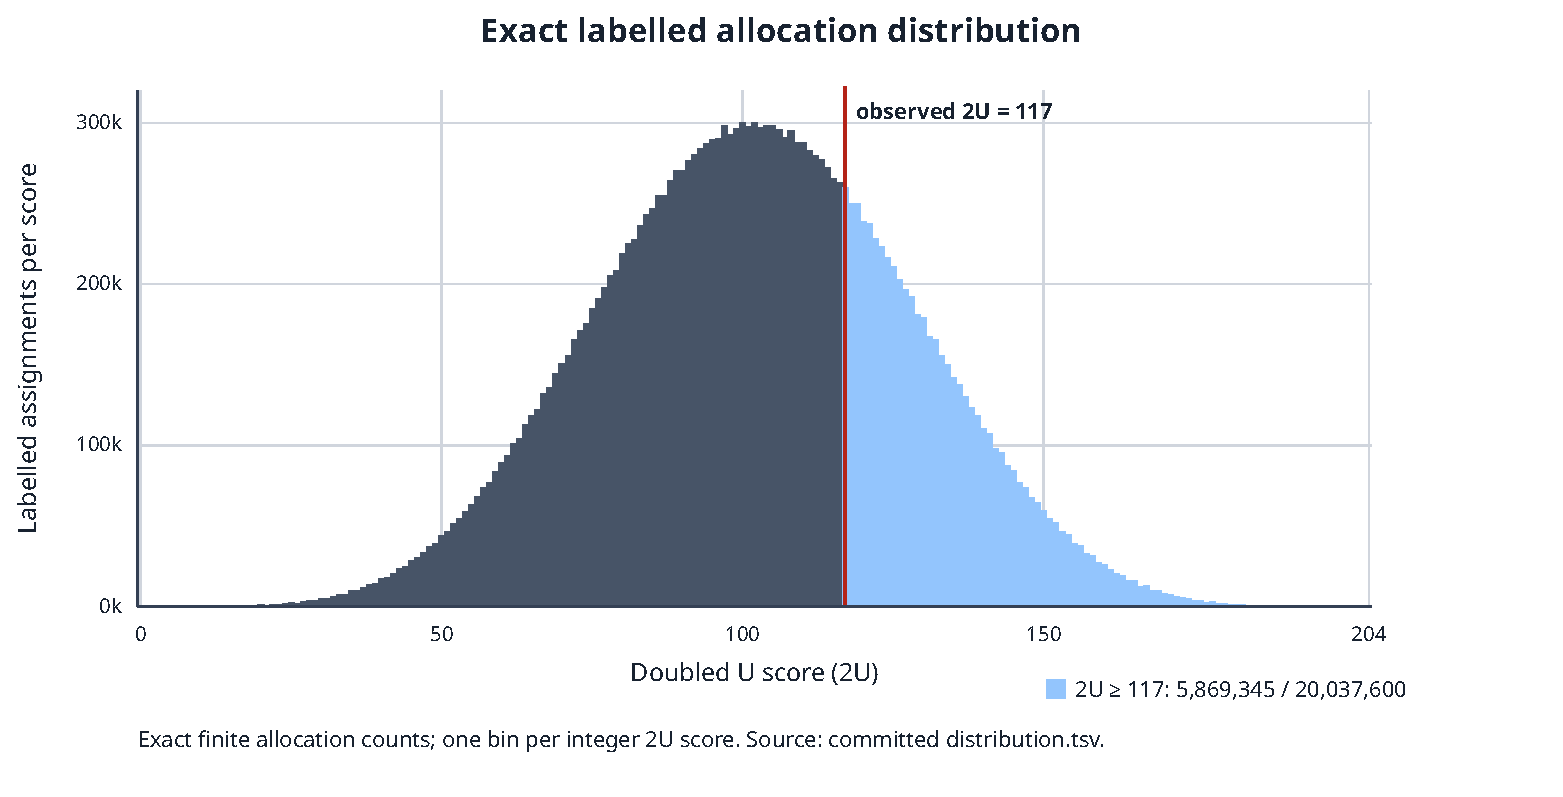
\includegraphics[width=0.92\linewidth]{figures/allocation-distribution.pdf}
\caption{Exact counts across all 20,037,600 labelled allocations. The vertical line marks the observed doubled score $2U=117$; the shaded inclusive upper tail contains 5,869,345 assignments. The distribution is derived from the committed exact TSV, not new sampling.}
\label{fig:allocation-distribution}
\end{figure}
``Higher'' means additional $>$ published. The observed fraction is
$(55+7/2)/102=117/204\simeq\PairFraction$. Exactly \TailNumerator{} assignments
have $2U\ge117$, giving the tail above. Figure~\ref{fig:allocation-distribution} shows the exact committed histogram and marks this observed threshold. It does not meet the source's nominal
0.05 replication threshold within this allocation model. A p-value
interpretation requires within-field label exchangeability; the exact finite
fraction itself assumes no real-curve sampling model. It neither proves an
absence of selection nor supplies a probability of historical manipulation.
\clearpage

\section{A public generator relationship is not a solver}
Suppose $G,Q\ne O$ lie in the same cyclic group of prime order $n$, with a
known relation $G=[s]Q$, $s\not\equiv0\pmod n$. For a target $P=[k]G$,
\[
 [s^{-1}\bmod n]P=[k]Q.
\]
Conversely a target $R=[k]Q$ maps to $[s]R=[k]G$. These public invertible
maps convert the DLP between bases; they do not supply the destination solver.
If a recipe derives $s$ from $b$, its conversion from $\mathbb F_p$ to a
scalar modulo $n$ must be specified. If $s=0$, it yields the identity and
fails the nonidentity-generator premise. This equivalence is not a general
security proof or a measured attack.

For $a=-3$, coordinates satisfy $b=y^2-x^3+3x\pmod p$: $x=0$ gives $y^2=b$,
and $x=1$ gives $y^2=b-2$. These field identities do not by themselves give
scalar logarithms. The supplied canonical points were assigned by a public
first-$x$ rule; they do not reveal historical unpublished generators.
RFC 5639 Appendix A.2, steps 12--13, gives a later standard example of a
smallest-$x$ point multiplied by a derived scalar~\cite{rfc}. Its subsequent
small-coordinate side-channel discussion concerns implementation behaviour.
It is not evidence that the 1997 NIST program used that construction.

\section{Verification and remaining evidence gap}
Source and input bindings were committed before allocation arithmetic at
\path{fc7bac88dc217d01c59ff750d973d2796ebba1b4}. Separate C++17 programs use
subset enumeration and rank dynamic programming; only the compiler and TSV
I/O are shared. All five files agree byte for byte. All ten phases pass as
specified: seven native zero exits and three deliberate corrupt-output
refusals with exit one. Full field/joint distributions, source checks,
commands, binaries and native statuses are retained. No new character, point
count, factorization, random draw, DLP or performance measurement is involved.

The exact existing-results audit uses the repository's local development
exception, explicitly recorded before execution. No checkpoint, S3 receipt or
gate on the separate sampling experiment is claimed passed. The requested
10000 accepted real prime-order curves per field and publication percentiles
remain unrun. The supported launch route still lacks a qualified PARI worker.
No original candidate visitation/acceptance logs are available. The combined
root/width/splitting fit, both weakness hypotheses and the historical cause
remain unresolved. No finite trait catalog exhausts all mathematical functions.

\begin{thebibliography}{9}\small
\bibitem{census} Prior verified census and scope report. Crypto revision
\path{c6d8897d7582fed39e8eb7fdd4e312a70d692532},
\path{research/nist_skip_criterion_20261025/broader_census_reanalysis_20261030}.
\bibitem{source} Prior lab report. Small-prime splitting: null, cutoff sweep
and held-out test. Crypto-autoresearcher revision
\path{3ff8c32c15f91b355d18e207d6044a1d2363499f},
\path{research/nist_seed_split_null_20261029/report.md}.
\bibitem{deviations} Same source revision and study, \path{DEVIATIONS.md},
deviations D1--D3. Original measurement admission is not retroactively repaired.
\bibitem{rfc} M. Lochter and J. Merkle. RFC 5639, Appendix A.2, March 2010.
\url{https://www.rfc-editor.org/rfc/rfc5639.txt}.
\end{thebibliography}
\end{document}
